\title{Pipeline Architecture}
\author{Brae Webb}
\date{\week{2}}

\maketitle

\section{Introduction}

Pipeline architectures take the attribute of modularity of a system to the extreme.
Pipeline architectures are composed of small well-designed components which can ideally be combined interchangeably.
In a pipeline architecture, input is passed through a sequence of components until the desired output is reached.
Almost every developer will have been exposed to software which implements this architecture.
Some notable examples are bash, hadoop, some older compilers, and most functional programming languages.

\begin{definition}[Pipeline Architecture]
    Components connected in such a way that the output of one component is the input of another.
\end{definition}


\begin{figure}[ht]
    \centering
\begin{tikzpicture}[>=latex']
    \tikzset{block/.style= {draw, rectangle, align=center,minimum width=2cm,minimum height=1cm},}

    \node [block] (input) {cat assignment.py};
    \node [block, right =2cm of input] (grep) {grep "f***"};
    \node [block, right =2cm of grep] (wc) {wc -l};
    \node [block, right =2cm of wc] (tee) {tee anger.txt};

    \path[draw,->]
                (input) edge (grep)
                (grep) edge (wc)
                (wc) edge (tee)
                ;
\end{tikzpicture}
\caption{An example of using bash's pipeline architecture to perform statistical analysis.}
\label{fig:bash-example}
\end{figure}

The de-facto example of a well-implemented pipeline architecture is bash,
we'll explore the philosophy that supports the architecture shortly.
The above diagram represents the bash command, \bash{cat assignment.py | grep "f***" | wc -l | tee anger.txt}.

\noindent
If you're unfamiliar with unix processes (start learning quick!),
\begin{description}
    \item[cat] Send the contents of a file to the output.
    \item[grep] Send all lines of the input matching a pattern to the output.
    \item[wc -l] Send the number of lines in the input to the output.
    \item[tee] Send the input to stdout and a file.
\end{description}

\section{Terminology}

As illustrated by Figure \ref{fig:pipe-filter}, a pipeline architecture consists of just two elements;

\begin{description}
    \item[Filters] modular software components, and
    \item[Pipes] the transmission of data between filters.   
\end{description}

\begin{figure}[ht]
    \centering
\begin{tikzpicture}[>=latex']
    \tikzset{block/.style= {draw, rectangle, align=center,minimum width=2cm,minimum height=1cm},}

    \node [block] (filter1) {Filter};
    \node [block, right =2cm of filter1] (filter2) {Filter};
    \node [block, right =2cm of filter2] (filter3) {Filter};

    \path[draw,->]
                (filter1) edge node[above] {Pipe} (filter2)
                (filter2) edge node[above] {Pipe} (filter3)
                ;
\end{tikzpicture}
\caption{A generic pipeline architecture.}
\label{fig:pipe-filter}
\end{figure}

\noindent Filters themselves are composed of four major types:

\begin{description}
    \item[Producers] Filters where data originates from are called producers, or source filters.
    \item[Transformers] Filters which manipulate input data and output to the outgoing pipe are called transformers.
    \item[Testers] Filters which apply selection to input data, allowing only a subset of input data to progress to the outgoing pipe are called testers.
    \item[Consumers] The final state of a pipeline architecture is a consumer filter, where data is eventually used.
\end{description}

The example in Figure \ref{fig:bash-example} shows how bash's pipeline architecture can be used to manipulate data in unix files.
Figure \ref{fig:bash-example-labelled} labels the bash command using the terminology of pipeline architectures.

\begin{figure}[H]
    \centering
\begin{tikzpicture}[>=latex']
    \tikzset{block/.style= {draw, rectangle, align=center,minimum width=2cm,minimum height=1cm},}

    \node [block,label=\color{gray}Producer] (input) {cat assignment.py};
    \node [block,label=\color{gray}Tester, right =2cm of input] (grep) {grep "f***"};
    \node [block,label=\color{gray}Transformer, right =2cm of grep] (wc) {wc -l};
    \node [block,label=\color{gray}Consumer, right =2cm of wc] (tee) {tee anger.txt};

    \path[draw,->]
                (input) edge (grep)
                (grep) edge (wc)
                (wc) edge (tee)
                ;
\end{tikzpicture}
\caption{Figure \ref{fig:bash-example} with labelled filter types.}
\label{fig:bash-example-labelled}
\end{figure}

\section{Pipeline Principles}
While the concept of a pipeline architecture is straightforward,
there are some principles which should be maintained to produce a well-designed and re-usable architecture.

\begin{definition}[One Direction Principle]
    Data should flow in one direction, this is the \textsl{downstream}.
\end{definition}

The data in a pipeline architecture should all flow in the same direction.
Pipelines should not have loops nor should filters pass data back to their \textsl{upstream} or input filter.
The data flow \textsl{is} allowed to split into multiple paths.
For example, Figure \ref{fig:analytics} demonstrates a potential architecture of a software which processes the stream of user activity on a website.
The pipeline is split into a pipeline which aggregates activity on the current page and a pipeline which records the activity of this specific user.

\begin{figure}
    \centering
    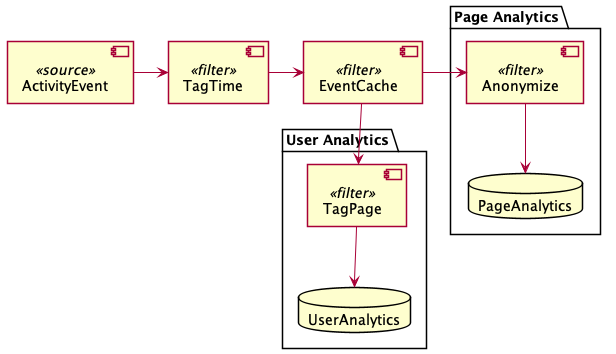
\includegraphics[width=0.8\textwidth]{diagrams/activity-tracking.png}
    \label{fig:analytics}
    \caption{Pipeline architecture for processing activity on a website for later analytics.}
\end{figure}

The One Direction Principle makes the pipeline architecture a poor choice for applications which require interactivity,
as the results aren't propagated back to the input source.
However, it is a good choice when you have data which needs processing with no need for interactive feedback.

\begin{definition}[Independent Filter Principle]
Testers and transformers should not rely on specific upstream or down-stream filters.
\end{definition}

In order to maintain the reusability offered by the pipeline architecture,
it is important to remove dependencies between individual filters.
Where possible, filters should be able to move around freely.
In the example architecture in Figure \ref{fig:analytics},
\todo{Filters needed between tags and databases}
the EventCache component should be able to work fine without
the TagTime component.
Likewise, EventCache should be able to process data if the
Anonymize filter is placed before it.

\section{Case Study: MapReduce}

One of the more prevalent uses of the pipeline architecture is the MapReduce pattern.
The MapReduce pattern was discovered in 2004 as a solution to the challenges which Google faced managing their search index \cite{mapreduce}.%
\footnote{Although the pattern was in use prior to their work\cite{mapreduce-critique}}%
MapReduce affords impressive parallelism inherit to the programming pattern.

The two key ideas of MapReduce, \textsl{map} and \textsl{reduce}, come from functional programming.\footnote{I \textsl{think}? Will consult with history textbook (Ian)}
Below are the generic types of the \textsl{map} and \textsl{reduce} functions in functional programming.

\begin{code}[language=lambda]{}
map : (type$_1$ -> type$_2$) -> type$_1 Seq$ -> type$_2 Seq$
map $f$ $xs$
reduce : (type$_1$ -> type$_1$ -> type$_1$) -> type$_1 Seq$ -> type$_1$ -> type$_1 Seq$
reduce $f$ $xs$ $initial$
\end{code}

If you're unfamiliar with this notation, the rough English translation is:
\begin{description}
    \item[map] The parameters of the \textsl{map} function are:
        \begin{enumerate}[label=(\alph*)]
            \item A function, $f$, which takes a parameter of type $\tau_1$ and returns a type $\tau_2$.
            \item A sequence of elements of type $\tau_1$.
        \end{enumerate}
        The return type of the \textsl{map} function is a sequence of elements of type $\tau_2$.
    \item[reduce] The parameters of the \textsl{reduce} function are:
        \begin{enumerate}[label=(\alph*)]
            \item A function, $f$, which takes two parameters both of type $\tau_1$ and returns a type $\tau_1$.
            \item A sequence of elements of type $\tau_1$.
            \item An initial accumulator value of type $\tau_1$
        \end{enumerate}
        The return type of the \textsl{reduce} function is a sequence of elements of type $\tau_1$.
\end{description}

The code snippet below uses the $map$ and $reduce$ functions
to perform the operations of the above bash example.
One important thing to note about the example below is the map operation on line 11.
Each application of the lambda function within the map operation is completely independent and could,
in theory, be executed simultaneously. 

\begin{code}[language=python,literate={{->}{{$\to$}}{2}{lambda}{{$\lambda$}}{1}},morekeywords={then}]{}
contents = read("assignment.py")

# filter relevant lines by rebuilding the list
contents = reduce(lambda xs x -> 
                    if x.contains("f***")
                        then x + xs
                        else xs,
                  contents)

# use map to count occurrences of word
contents = map(lambda line -> line.count("f***"), contents)

# use reduce to sum list of counts
contents = reduce(lambda total curr -> total + curr, contents, 0)

write("anger.txt", contents)
\end{code}

So by design, code written in this pattern can process data simultaneously.
Tools such as \link{Hadoop}{https://hadoop.apache.org/} are able to take advantage of this to distribute computation automatically.

\begin{extra}
Using the terminology of a pipeline architecture, what filters do the \textsl{map} and \textsl{reduce} operators correspond to?
\end{extra}

\begin{extra}
How would you improve the efficiency of the code snippet above?
\end{extra}

\section{Case Study: Compilers}

An interesting case study of the pipeline architecture is a compiler.%
\footnote{You don't need to understand the phases of a compiler --- two data structures, the Symbol Table and AST, are transformed in each compiler phase.}
As a foundational technology, compilers have undergone rigorous refinement and are perhaps the most well studied type of software.
Modern compilers have well-defined modular phases as illustrated by Figure \ref{fig:compiler-architecture},
each phase of a compiler transforms the representation of the program until the target program is produced.

\begin{figure}[H]
    \centering
\begin{tikzpicture}[>=latex']
    \tikzset{block/.style= {draw, rectangle, align=center,minimum width=2cm,minimum height=1cm},}

    \node (src) {Source Program};
    \node [block, below =1cm of src] (lex) {Lexical Analyzer};
    \node [block, right =1cm of lex] (syn) {Syntax Analyzer};
    \node [block, right =1cm of syn] (sem) {Semantic Analyzer};
    \node [block, below =1cm of sem] (opt) {Code Optimizer};
    \node [block, left =1cm of opt] (gen) {Code Generator};
    \node [below =1cm of gen] (tar) {Target Program};

    \path[draw,->]
                (src) edge (lex)
                (lex) edge (syn)
                (syn) edge (sem)
                (sem) edge (opt)
                (opt) edge (gen)
                (gen) edge (tar)
                ;
\end{tikzpicture}
\caption{Typical phases of a compiler.}
\label{fig:compiler-architecture}
\end{figure}

However, a compiler is not well suited to use a pipeline architecture.
In general, the modules of a pipeline architecture should be independent of their input source.
This is not the case in compilers, as each phase relies on the completion of the previous phase.
As a result, the input dependencies of a compiler make it too restrictive for a true pipeline architecture.

Instead, compilers are often built as a hybrid of a pipeline architecture and the \textsl{Blackboard Architecture}.
The blackboard architecture consists of;
\begin{itemize}
    \item a knowledge base, the `blackboard',
    \item knowledge sources which use and update the knowledge base, and
    \item a control component to coordinate the operation of knowledge sources.
\end{itemize}

In modern compilers, the data which would be passed through pipes, the Symbol Table and AST,
are used and updated by each phase.
They are subsequently used as the `blackboard'.
Each phase is considered a knowledge source which uses the knowledge base to transform and update the knowledge base.
Finally, in this hybrid, the control component is not required as the sequence of phase execution in a pipeline coordinates operation.
Figure \ref{fig:compiler-architecture-sym} illustrates this proposed architecture.
Of course, there are many compilers out there, many of them deviate from this architectural hybrid.

\begin{figure}[H]
    \centering
\begin{tikzpicture}[>=latex']
    \tikzset{block/.style= {draw, rectangle, align=center,minimum width=2cm,minimum height=1cm},}

    \node (src) {Source Program};
    \node [block, below =1cm of src] (lex) {Lexical Analyzer};
    \node [block, right =1cm of lex] (syn) {Syntax Analyzer};
    \node [block, right =1cm of syn] (sem) {Semantic Analyzer};
    \node [block, below =3cm of sem] (opt) {Code Optimizer};
    \node [block, left =1cm of opt] (gen) {Code Generator};
    \node [below =1cm of gen] (tar) {Target Program};

    \node [block, below =1cm of syn] (sym) {Symbol Table\\AST};

    \path[draw,->]
                (src) edge (lex)
                (lex) edge (syn)
                (syn) edge (sem)
                (sem) edge (opt)
                (opt) edge (gen)
                (gen) edge (tar)
                ;

    \path[draw,<->] (lex) edge (sym);
    \path[draw,<->] (syn) edge (sym);
    \path[draw,<->] (sem) edge (sym);
    \path[draw,<->] (opt) edge (sym);
    \path[draw,<->] (gen) edge (sym);
\end{tikzpicture}
\caption{Modern phases of a compiler.}
\label{fig:compiler-architecture-sym}
\end{figure}
